This section describes the instance of \NAME\ proposed in this paper, using PKSs and and LTL. We first show how we modified the theorem prover framework presented in Section~\ref{sec:preliminaries} to support PKSs and how it is integrated with the three-valued model checker. We further analyze the case of thorough semantics, which is more appealing in practice, and discuss to what extent and how the framework can be used in such a case.
% and the theorem prover;
%\item the correctness of the integrated framework considering the three-valued and the thorough LTL semantics also for the subset of self-minimizing LTL formulae.
%\end{enumerate*}




\subsection{Adapting the theorem prover.}
\label{sec:adapting}
The deductive verification framework presented in~\cite{peled2001model}  exploits the product between a state labeled transition system and  a GBA \gba\ obtained by $\lnot\phi$ to generate the proof.
To enable the algorithm to work on KSs and BAs, 
we describe
%it is necessary to specify
 how to associate LTL formulae with each state of the BA and how to identify failed states of the product automaton.

\vskip 0.05in  
\textbf{Identification of the formulae that hold in the states of  the BA.}
We assume that the degeneralization procedure~\cite{clarke1999model}, that converts the GBA  \gba\
%$\mathcal{G}$ 
 into an equivalent BA \ba\
 %$\mathcal{A}$,
  behaves as follows: when a new state $q$ of 
  %$\mathcal{A}$
  \ba\ is created from a state $q^\prime$ of 
  \gba ,
  %$\mathcal{G}$, 
the formulae $\eta(q^\prime)$ and $\mu(q^\prime)$ are also associated to $q$.

\vskip 0.05in  
\textbf{Identification of failed states.} 
Following the procedure mentioned in Section~\ref{sec:preliminaries}, the product automaton 
%$M\otimes\mathcal{A}$
$M\otimes \ba$
 between the KS $M$ and the BA 
 %$\mathcal{A}$ 
\ba\ is modified to also generate \emph{failed states}.
Specifically, the product is computed using the rules~\ref{eq:classicalTransition} and~\ref{eq:failedTransition}.
%
\vspace{-1cm}
\begin{multicols}{2}
\begin{equation}
\label{eq:classicalTransition}
 \inferrule{s\rightarrow t \land q \xrightarrow{L(t)}p}{\langle s,q \rangle \rightarrow \langle t,p \rangle}  
\end{equation}\break
\begin{equation}
\label{eq:failedTransition}
 \inferrule{s\rightarrow t \land q \xrightarrow{\cancel{L(t)}}p}{\langle s,q \rangle \dashrightarrow \langle t,p \rangle}  
\end{equation}
\end{multicols}
%
Rule~\ref{eq:classicalTransition} is the classical rule used to compute the product automaton. 
It specifies that the state of the product $\langle s,q \rangle$  moves to $\langle t,p \rangle$ only if the transition $q \xrightarrow{L(t)}p$ that moves the BA from  $q$ to $p$ has the same label of the state $t$ of $M$.
Rule~\ref{eq:failedTransition} specifies how to compute failed states.
It states that the failed state $\langle t,p \rangle$ is generated in the product  when a transition  that moves the BA 
%$\mathcal{A}$
 \ba\ from $q$ to $p$ is labelled differently with respect to the state $t$ reached by the model $\mathcal{M}$ when the transition $s\rightarrow t$ is fired.
This is indicated using the notation $q \xrightarrow{\cancel{L(t)}}p$.
For this reason, the transition $\langle s,q \rangle \dashrightarrow \langle t,p \rangle$  from $\langle s,q \rangle $ to $\langle t,p \rangle$ is dashed.
Let us consider the product presented in Figure~\ref{fig:productOpt}  computed from the KS $M_{opt}$ obtained from the PKS in Figure~\ref{fig:model} and the BA of Figure~\ref{fig:property}.
The transition $\langle s_0, q_0 \rangle$ to  $\langle s_1, q_1 \rangle$ of the product presented in Figure~\ref{fig:productOpt} is dashed, since the proposition $\overline{g}$ is false in $s_1$, while the labeling of the transition from $q_0$ to $q_1$ requires $\overline{g}$ to be true for the transition to be performed.

The set 
%$\mathcal{F}(M\otimes\mathcal{A})$ 
 $\mathcal{F}(M\otimes \ba)$ of the \emph{failed states} contains the states $\langle t, p \rangle$ obtained by applying rule~\ref{eq:failedTransition}.
Note that, as stated in Section~\ref{sec:preliminaries}, each failed state $\langle s, q \rangle$ is such that $s \models \mu(q) $.
For example, the state $\langle s_1, q_1 \rangle$ of the product  presented in Figure~\ref{fig:productOpt} is a failed state.
Indeed, $s_1$ satisfies the property $\mu(q_1)= g \LTLor \LTLnext \LTLfinally g$ associated with the state $q_1$.



%%%%%%%%%%%%%%
\begin{theorem}
\label{th:deductivecorrecteness}
The deductive verification procedure is correct.
\end{theorem}

\begin{proof}
We show that the states identified as \emph{failed}  correspond to the ones that would be identified using~\cite{peled2001model}. 
In~\cite{peled2001model}, a state $\langle t, p \rangle$ is failed if the propositional assignment of $t$ does not satisfy the conditions specified in the state $p$. 
It is well known~\cite{gerth1996ltl2ba,clarke1999model}, that a GBA \gba\ associated with $\phi$ is such that
\begin{enumerate*}[label={(\arabic*)}]
\item all the transitions $(q,\alpha, p) \in \Delta$ that reach a state $p$ of the GBA have the same label $\alpha$ and that
\item a transition $(q,\alpha, p) \in \Delta$ is in the GBA  if and only if $\alpha$ satisfies the conjunction of the negated and non negated propositions that hold in the state $p$.
\end{enumerate*}
By construction, the latter of these properties also holds in the BA obtained from the GBA by applying the degeneralization procedure~\cite{clarke1999model}.
Thus, since all the transitions that reach $p$ are labelled with $\alpha$, a transition $\langle s,q \rangle \dashrightarrow' \langle t,p \rangle$ is added to the product automaton if and only if the propositional assignment of $t$ does not satisfy the propositional assignment specified in the state $p$. 
Furthermore, BAs acceptance condition is a special case of fairness condition used in~\cite{peled2001model}. 
Thus, the proposed deductive verification procedure is a special case of~\cite{peled2001model}, with regard to acceptance.\qed
\end{proof}

\begin{figure}[t]
\begin{minipage}[b]{.5\textwidth}
  \begin{figure}[H]
\centering




\begin{tikzpicture}[scale=0.33] %[x={10.0pt},y={10.0pt}]

\node[statep, initial, initial text={}, initial where=above] (s0q0) 
%[label={[yshift=-1.1cm,xshift=0cm]\scriptsize $\{q_0\}$},font=\scriptsize] {$\langle s_0,q_0\rangle$}; 
[font=\scriptsize] {$\langle s_0,q_0\rangle$}; 
\node[statep,  initial, initial text={}, initial where=above] (s0q1) 
%[below = 0.6cm of s0q0,label={[yshift=-1.1cm,xshift=0.5cm]\scriptsize $\{q_1\}$},font=\scriptsize] {$\langle s_0,q_1\rangle$}; 
[below = 0.6cm of s0q0,font=\scriptsize] {$\langle s_0,q_1\rangle$}; 

\node[statep] (s1q0) 
%[left = 0.4cm of s0q0,label={[yshift=-1.1cm,xshift=0cm]\scriptsize $\{q_0\}$},font=\scriptsize] {$\langle s_1,q_0\rangle$}; 
[left = 0.4cm of s0q0,font=\scriptsize] {$\langle s_1,q_0\rangle$}; 
\node[statep] (s1q1) 
%[below = 0.6cm of s1q0,label={[yshift=-1.1cm,xshift=0.5cm]\scriptsize $\{q_1\}$},font=\scriptsize] {$\langle s_1,q_1\rangle$}; 
[below = 0.6cm of s1q0,font=\scriptsize] {$\langle s_1,q_1\rangle$}; 

\node[statep] (s2q0) 
%[right = 0.4cm of s0q0,label={[yshift=-1.1cm,xshift=0cm]\scriptsize $\{q_0\}$},font=\scriptsize] {$\langle s_2,q_0\rangle$}; 
[right = 0.4cm of s0q0,font=\scriptsize] {$\langle s_2,q_0\rangle$}; 
\node[statep] (s2q1) 
%[below = 0.6cm of s2q0,label={[yshift=-1.1cm,xshift=-0.5cm]\scriptsize $\{q_1\}$},font=\scriptsize] {$\langle s_2,q_1\rangle$}; 
[below = 0.6cm of s2q0,font=\scriptsize] {$\langle s_2,q_1\rangle$}; 

%%LABELS for steps
\node[empty] (step3u) [above = 0.155cm of s0q0] {}; 
\node[empty] (step1u) [below = 0.155cm of s0q1] {}; 
\node[emptynode] (step3) [left = 1.9cm of step3u] {\tiny Step 3}; 
\node[emptynode] (step1) [left = 1.9cm of step1u] {\tiny Step 1}; 
\node[emptynode] (step1b) [right = 1.9cm of step1u] {\tiny Step 1}; 
\node[emptynode] (step2) [right= 1.1cm of step1] {\tiny Step 2};


\path[->]      
(s0q0) edge [bend left=15] node []{} (s1q0) 
(s1q0) edge [bend left=15] node []{} (s0q0)  

(s0q0) edge [bend left=15] node []{} (s2q0) 
(s2q0) edge [bend left=15] node []{} (s0q0)  

(s1q0) edge [bend right=5] node []{} (s0q1)
(s2q0) edge [bend left=5] node []{} (s0q1)

(s0q0) edge [bend left=5,dashed] node []{} (s1q1)
(s0q0) edge [bend right=5,dashed] node []{} (s2q1)

(s0q1) edge [bend left=5,dashed] node []{} (s1q1) 
(s0q1) edge [bend right=5,dashed] node []{} (s2q1) 
;    

\begin{pgfonlayer}{background}

%FAILED
\filldraw [line width=2mm,join=round,black!5]
(s1q1.south -| s1q1.west) rectangle (s1q1.north -| s1q1.east);
\filldraw [line width=2mm,join=round,black!5]
(s2q1.south -| s2q1.west) rectangle (s2q1.north -| s2q1.east);

%SUCCESSORS
\filldraw [line width=2mm,join=round,black!20]
(s0q1.south -| s0q1.west) rectangle (s0q1.north -| s0q1.east);

%INDUCTION
\filldraw [line width=2mm,join=round,black!35]
(s1q0.south -| s1q0.west) rectangle (s2q0.north -| s2q0.east);

\end{pgfonlayer}


\end{tikzpicture}

\caption{Product $I_{opt}=M_{opt}\otimes\mathcal{A}_{\lnot\phi_2}$}
\label{fig:productOpt}
 \end{figure}
\end{minipage}%
\begin{minipage}[b]{.5\textwidth}
  \begin{figure}[H]
\centering
\begin{tikzpicture}[scale=0.33] %[x={10.0pt},y={10.0pt}]

\node[statep, initial, initial text={}, initial where=above] (s0q0) 
%[label={[yshift=-1.1cm,xshift=0cm]\scriptsize $\{q_0\}$},font=\scriptsize] {$\langle s_0,q_0\rangle$}; 
[font=\scriptsize] {$\langle s_0,q_0\rangle$}; 
\node[statep,  initial, initial text={}, initial where=above] (s0q1) 
%[below = 0.6cm of s0q0,label={[yshift=-1.1cm,xshift=0cm]\scriptsize $\{q_1\}$},font=\scriptsize] {$\langle s_0,q_1\rangle$}; 
[below = 0.6cm of s0q0,font=\scriptsize] {$\langle s_0,q_1\rangle$}; 

\node[statep] (s1q0) 
%[left = 0.4cm of s0q0,label={[yshift=-1.1cm,xshift=0cm]\scriptsize $\{q_0\}$},font=\scriptsize] {$\langle s_1,q_0\rangle$}; 
[left = 0.4cm of s0q0,font=\scriptsize] {$\langle s_1,q_0\rangle$}; 

\node[statep] (s2q0) 
%[right = 0.4cm of s0q0,label={[yshift=-1.1cm,xshift=0cm]\scriptsize $\{q_0\}$},font=\scriptsize] {$\langle s_2,q_0\rangle$}; 
[right = 0.4cm of s0q0,font=\scriptsize] {$\langle s_2,q_0\rangle$}; 
\node[statep] (s2q1) 
%[below = 0.6cm of s2q0,label={[yshift=-1.1cm,xshift=0cm]\scriptsize $\{q_1\}$},font=\scriptsize] {$\langle s_2,q_1\rangle$}; 
[below = 0.6cm of s2q0,font=\scriptsize] {$\langle s_2,q_1\rangle$}; 

\path[->]      
(s0q0) edge [bend left=15] node []{} (s1q0) 
(s1q0) edge [bend left=15] node []{} (s0q0)  

(s0q0) edge [bend left=15] node []{} (s2q0) 
(s2q0) edge [bend left=15] node []{} (s0q0)  

(s1q0) edge [bend right=5] node []{} (s0q1)
(s2q0) edge [bend left=5] node []{} (s0q1)

%(s0q0) edge [bend left=5,dashed] node []{} (s1q1)
(s0q0) edge [bend right=5] node []{} (s2q1)

%(s0q1) edge [bend left=5,dashed] node []{} (s1q1) 
(s0q1) edge [bend left=15] node []{} (s2q1) 
(s2q1) edge [bend left=15] node []{} (s0q1) 
;    

\end{tikzpicture} % pic 1
\caption{Product $I_{pes}=M_{pes}\otimes\mathcal{A}_{\lnot\phi_2}$}
\label{fig:productPess}
 \end{figure}
\end{minipage}%
\end{figure}
\subsection{Integrating the model checker and the theorem prover}
\label{sub:integrating}
Figure~\ref{Fig.3vdvinstance} presents an instance of \NAME\ obtained as an integration of a model checker for PKSs and LTL based on three-valued semantics and the theorem prover presented in Section~\ref{sec:adapting}. The circled numbers in Figure~\ref{Fig.3vdvinstance} indicate how this specific instance is plugged into \NAME\ in Figure~\ref{Fig.3vdv}.






The three-valued model checker presented in Section~\ref{sec:preliminaries} is used by \NAME\  to check the satisfaction of the property of interest.
Specifically, it runs twice a classical two-valued model checker, considering first the optimistic approximation $M_{opt}$, then the pessimistic approximation $M_{pes}$ of the PKS $M$.
When $M_{opt}$ is evaluated, if a counterexample is found, this is returned as output of \NAME .
Otherwise, \NAME\ verifies $M_{pes}$. 
If the property is satisfied, it means that no violating nor possibly violating behaviors have been identified.
Thus, \NAME\ executes the theorem prover that produces a proof that explains why no counterexample has been found in the pessimistic approximation.
Otherwise, the property is possibly satisfied.
In this case, \NAME\ returns the possible counterexample and runs the theorem prover on $M_{opt}$ to compute a proof that specifies why a definitive counterexample has not be found.




\begin{figure}[t]
\begin{center}         
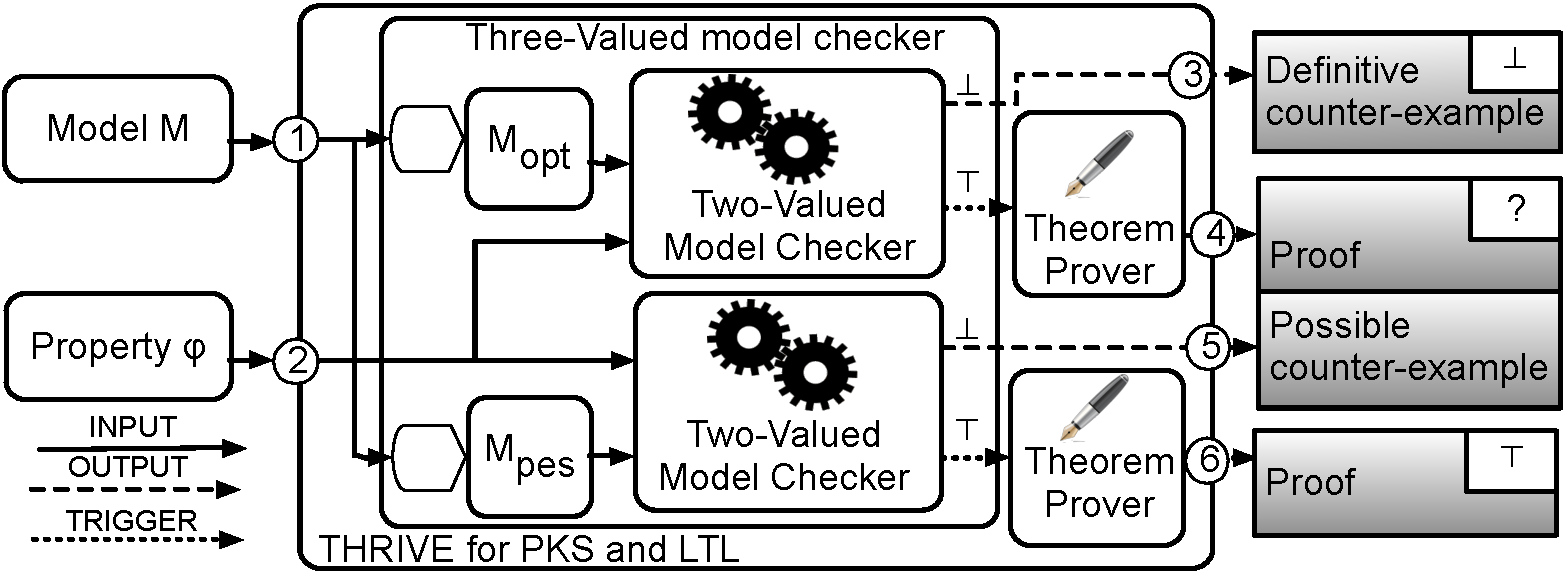
\includegraphics[width=\linewidth]{./images/atvaFigPKS.pdf}
\end{center}
\caption{\NAME\ for PKS and LTL.}  
\label{Fig.3vdvinstance}
\end{figure}



\textbf{Example}
%\emph{Consider properties $\phi_1$, $\phi_2$ and $\phi_3$ of the crossing semaphore example. They are satisfied, possibly satisfied and not satisfied, respectively, by the model $M$ of Figure~\ref{fig:model}.}
\emph{Properties $\phi_1$, $\phi_2$ and $\phi_3$ of the crossing semaphore example are satisfied, possibly satisfied and not satisfied by the model $M$ of Figure~\ref{fig:model}.}

\emph{
Property $\phi_2$.
The products between the optimistic and pessimistic approximation of the model $M$ and the BA automaton $\mathcal{A}_{\neg \phi_2}$ are presented in Figures~\ref{fig:productOpt} and~\ref{fig:productPess}.
\NAME\ explores $I_{pes}$ and returns the possible counterexample $(s_0, s_2)^\omega$.
Specifically,  by looping an infinite number of times on states $s_0$ and $s_2$ the green light is never turned on.
Since the property $\phi_2$ is possibly satisfied, the search of a definitive counterexample in the product automaton $I_{opt}$ (Figure~\ref{fig:productOpt}) fails.
%\NAME\ uses the product automaton $I_{opt}$ to compute a proof that explains the motivation.
%The obtained proof is presented in Table~\ref{table:proof}.
\NAME\ uses the product automaton $I_{opt}$ to compute a proof (Table~\ref{table:proof}) that explains the motivation.
The states that are analyzed in different steps are circled  in Figure~\ref{fig:productOpt} through different grey frames.
(\emph{Step1}). \NAME\ analyzes the failed states.
Given a failed state $\langle s, q \rangle$, since in this state the search for a counterexample fails, the formula associated with the state $q$ of $\mathcal{A}_{\lnot\phi_2}$ holds in $s$.
For example, since the state $\langle s_1, q_1 \rangle$ of $I_{opt}$ is a failed state, the formula $green \LTLor \LTLnext \LTLfinally green$ (valid in $q_1$) is satisfied by the model state $s_1$.
This formula is effectively true in $s_1$ since the green light is on.
(\emph{Step2}). Since all the successors of $\langle s_0, q_1 \rangle$ satisfy $green \LTLor \LTLnext \LTLfinally green$, it is possible to deduce that this property is also satisfied in $s_0$.
(\emph{Step3}). 
%The induction rule is applied considering the strongly connected component  $\left \{ \langle s_0, q_0 \rangle, \langle s_1, q_0 \rangle, \langle s_2, q_0 \rangle \right \}$.
%The rule allows to conclude that $s_0$ satisfies the property $\LTLnext \LTLglobally \LTLfinally green$.
The induction rule is applied considering the strongly connected component  $\left \{ \langle s_0, q_0 \rangle, \langle s_1, q_0 \rangle, \langle s_2, q_0 \rangle \right \}$ and  allows concluding that $s_0$ satisfies the property $\LTLnext \LTLglobally \LTLfinally green$.
(\emph{Step4}). \NAME\ applies the conjunction rule to $s_0$.
Since $s_0$ satisfies both $\LTLnext \LTLglobally \LTLfinally green$ and $green \LTLor \LTLnext \LTLfinally green$, it is possibly to deduce that $s_0$ satisfies the property $\phi_2$.
This provides an interesting insight to the designer: if she/he turns the green light on in $s_2$ the property becomes satisfied. The proof clearly states why.}

\emph{Property $\phi_3$. \NAME\ returns the counterexample $(s_0, s_1)^\omega$.
The counterexample specifies that by looping an infinite number of times on states $s_0$ and $s_1$ the green light is not permanently  on after the red. }

\emph{Property $\phi_1$. \NAME\  produces a proof that highlights how and why a definite counterexample is not found in the graph. First, it identifies the states $\langle s_0, q_1 \rangle$ and $\langle s_2, q_1 \rangle$ as failed. The conclusions found on these states are propagated to the state $\langle s_1, q_1 \rangle$. All the successors of the SCC formed by the product states related to the property state $q_0$ are analyzed. Finally, conclusions are drawn also on this SCC. 
The proof is omitted for space reasons.
}



\begin{table}[t]
\centering
\caption{Proof that $\phi_2$ is not violated.}
\label{table:proof}
\begin{tabular}[b]{ | P{2.5cm} | P{2.1cm} | P{3.3cm} | P{3cm} |  }
\hline
\emph{Step 1} &
\emph{Step 2} &
\emph{Step 3} &
\emph{Step 4}\\
\hline
%%\multicolumn{4}{|c|}{Steps}  \\
%% \hline
\textbf{Fail} & 
\textbf{Successors} &
\textbf{Induction} &
\textbf{Conjunction}\\
 \hline
\mbox{ $\langle s_2,q_1\rangle, \langle s_1,q_1\rangle$}
 &
 $\langle s_0,q_1\rangle$ 
 &
 $\mathcal{X}=\{\langle s_0,q_0\rangle,$ $ \langle s_1,q_0\rangle,\langle s_2,q_0\rangle\}$\newline
 $Exit(\mathcal{X})=\{\langle s_0,q_1\rangle, $ $ \langle s_1,q_1\rangle,\langle s_2,q_1\rangle\}$
 &
The initial state $s_0$ \\	
 \hline
  \inferrule{\langle s_1,q_1 \rangle  \in \mathcal{F}(I_{opt})\\
 \langle s_2,q_1 \rangle \in \mathcal{F}(I_{opt})
}
{ s_1, s_2\models g \LTLor \LTLnext \LTLfinally g }
  & 
 \inferrule{s_0\rightarrow\{s_1,s_2\} \\
 s_1\models g \LTLor \LTLnext \LTLfinally g \\
 s_2\models g \LTLor \LTLnext \LTLfinally g }
 {s_0\models g \LTLor \LTLnext \LTLfinally g} 
  &
\mbox{   \inferrule{ 
 s_0,s_1,s_2\models g \LTLor \LTLnext \LTLfinally g \\
s_0\rightarrow \{s_1,s_2 \} \\\\
 s_1\rightarrow \{s_0 \} \\\\
 s_2\rightarrow \{s_0 \}   
   }
{s_0,s_1,s_2\models \LTLnext \LTLglobally \LTLfinally g }}
  &
\inferrule{
 s_0\models \LTLnext \LTLglobally \LTLfinally g \\
  s_0\models g \LTLor \LTLnext \LTLfinally g \\
 \LTLnext \LTLglobally \LTLfinally g \LTLand  (g \LTLor  \LTLnext \LTLfinally g)\rightarrow \phi_2 }
 {s_0\models \phi_2}
\\  
\hline

\end{tabular}
\end{table}

\subsection{Thorough semantics and \NAME}
As stated in Section~\ref{sec:preliminaries},  three-valued semantics does not always behave in accordance with the natural intuition~\cite{bruns2000model}.
When $\phi$ possibly holds in $M$,   it is desirable that there exist two completions $M^\prime$ and $M^{\prime\prime}$ of $M$  such that $M^\prime$ satisfies  $\phi$  and   $M^{\prime\prime}$ violates $\phi$.
This property is not ensured by the three-valued semantics, and is the motivation that leads to introduce thorough LTL semantics. Hereafter, we discuss how the adoption of thorough semantics would affect the use of the \NAME\ framework.

Given a PKS  $M$ and a property  $\phi$,  \NAME\ produces the following outputs:

\noindent \emph{Property is satisfied.}
%In this case, \NAME\ works correctly. 
\NAME\ works correctly. 
A property $\phi$ that evaluates to $\LTLtrue$ under three-valued semantics is also satisfied under thorough semantics.
Thus, the  verification result is correct.
Also the proof is correct since it shows that any completion of $M$ satisfies $\phi$. 

\noindent \emph{Property is not satisfied.}
%In this case, \NAME\ works correctly. 
 \NAME\ works correctly. 
When the model checker returns a $\LTLfalse$ value, the counterexample shows a behavior that violates $\phi$.
A property $\phi$  that is not satisfied considering the three-valued semantics, is also not satisfied considering the thorough semantics.
%Thus, the counterexample is a correct counterexample that proves the existence of a completion of $M$ that violates $\phi$.
Thus, the counterexample is correct and proves the existence of a completion of $M$ that violates $\phi$.
 
\noindent \emph{Property is possibly satisfied.}
%This case is not handled by \NAME\ correctly for all LTL properties.
 \NAME\ does not work correctly  for all LTL properties. 
When the three-valued model checker returns  $?$  the property is possibly satisfied considering the three-valued semantics but no conclusion can be drawn based on thorough semantics.
Indeed, there are cases in which a $?$ is returned, but all the completions of the model either satisfy or do not satisfy $\phi$. 
The computed counterexample and proof can be spurious under the thorough semantics.


%In this case, if a correct result is required, the use of a generalized model checking procedure~\cite{bruns2000model} (not discussed here) becomes necessary. 
%Since when a property $\phi$ is evaluated to $?$ there could exist a completion that violates $\phi$, the produced proof is not correct.

%
%
%Correctness is analyzed by comparing the results returned by \NAME\ with the  results  that would be returned considering the thorough LTL semantics.
%We stated that a model checking result---the verification result, the counterexample or the possible counterexample---is \emph{correct} (\validCounterexample ) if it corresponds to the results that would be obtained considering the thorough LTL semantic.
%Otherwise, it is \emph{incorrect} (\spuriosCounterexample), i.e., the counterexample can be spurious.
%We stated that a proof generated by \NAME\ is \emph{correct} (\validProof) if it proves the satisfaction/possibly satisfaction of a property considering the thorough LTL semantics. 
%Otherwise, it is \emph{incorrect} (\notvalidProof ).
%Table~\ref{tab:results} shows the comparison. 
%The rows of the table specify whether \NAME\ states that the property of interest is satisfied ($\LTLtrue$), possibly satisfied ($?$) or not satisfied ($\LTLfalse$).
%If the property is satisfied/possibly satisfied Table~\ref{tab:results} considers the correctness of the verification result ($\LTLtrue$, $?$ or $\LTLfalse$) and the proof.
%If the property is not satisfied only the correctness of the verification result is considered since no proof is produced.
%The correctness of the framework w.r.t. LTL properties is presented by the column with labeled as LTL.

%\textbf{Property satisfied.}
%When a property $\phi$ is evaluated to $\LTLtrue$ considering the three-valued semantics, it is also satisfied considering the thorough semantics.
%Thus, the  verification result is correct.
%Also the proof is correct since it shows that any completion of $M$ satisfies $\phi$. 
%
%\textbf{Property not satisfied.}
%When the model checker returns a $\LTLfalse$ value, the counterexample shows a behavior that violates $\phi$.
%A property $\phi$  that is not satisfied considering the three-valued semantics, is also not satisfied considering the thorough semantics.
%Thus, the counterexample is a correct counterexample that proves the existence of a completion of $M$ that violates $\phi$.
% 
%\textbf{Property possibly satisfied.}
%When the three-valued model checker returns a $?$ value the property is possibly satisfied considering the three-valued semantics but no conclusion can be achieved by considering the thorough semantics.
%Indeed, there are cases in which a $?$ is returned but all the completions of the model either satisfy or do not satisfy the property of interest. 
%The computed counterexample can be a spurious counterexample under the thorough semantics.
%The corresponding cell in Table~\ref{tab:results} is marked with a \spuriosCounterexample\ symbol meaning that the counterexample is not correct.
%In this case, if a correct result is required, the use of a generalized model checking procedure~\cite{bruns2000model} (not discussed here) becomes necessary. 
%Since when a property $\phi$ is evaluated to $?$ there could exist a completion that violates $\phi$, the produced proof is not correct.


%
%\begin{table}[t]
%\centering
%\caption{LTL and self-minimizing LTL validity of the framework outputs.}
%\label{tab:results}
%\begin{tabular}{   c  c | c | c | }
%\cline{1-4}
%  \multicolumn{1}{| c }{Result} & \multicolumn{1}{| c |}{Type of Output} & \multicolumn{1}{c |}{LTL} & \multicolumn{1}{c |}{Self-minimizing LTL} \\
%\cline{1-4} 
%  \multicolumn{1}{| c }{\multirow{2}{*}{$\LTLtrue$}} &  \multicolumn{1}{| c |}{Verification result} & \multicolumn{1}{ c |}{\validCounterexample}  & \validCounterexample  \\
%    \cline{2-4}
% \multicolumn{1}{| c }{} &  \multicolumn{1}{| c |}{Proof} & \validProof  & \validProof  \\
%  \cline{1-4}
%  \multicolumn{1}{| c }{\multirow{2}{*}{$?$}} &  \multicolumn{1}{| c |}{Verification result}  & \multicolumn{1}{ c |}{\spuriosCounterexample} & \validCounterexample  \\
%  \cline{2-4}
%  \multicolumn{1}{| c }{} &  \multicolumn{1}{| c |}{Proof} & \notvalidProof\  & \validProof  \\
%   \cline{1-4}
% \multicolumn{1}{| c }{$\LTLfalse$} & \multicolumn{1}{| c |}{Verification result} &  \multicolumn{1}{ c |}{\validCounterexample} & \validCounterexample   \\
% \hline
%\end{tabular}
%\end{table}
% 
%
\textbf{Example.}
\emph{The results obtained for $\phi_1$ and $\phi_3$ of the crossing semaphore example are correct both considering the three-valued and the thorough semantics. 
Since $\phi_1$ is satisfied, the proof is a correct proof that justifies why all the completions of the model presented in Figure~\ref{fig:modelmot} satisfy $\phi_1$.
The counterexample  returned for $\phi_3$ is correct, i.e., all the completions of the model presented in Figure~\ref{fig:modelmot} exhibit the behavior returned as a counterexample.}


\vskip 0.05in  
\textbf{Self-minimizing LTL formulae.} 
Self-minimizing LTL formulae are a subset of LTL formulae that present an interesting property:  three-valued and  thorough semantics are equivalent, i.e., if $\phi$ is self-minimizing, then $[(M, s) \models \phi]=[(M, s) \models \phi]_t$.
Therefore, the three-valued model checking framework presented in Section~\ref{sec:preliminaries} produces a result that is correct also considering the thorough semantics. 
For this reason, whenever the three-valued model checker returns $?$,  the proof and the possible counterexample produced by \NAME\ are also correct  under the thorough semantics. In~\cite{godefroid2005MCvsGMC}, the authors propose a first grammar for this LTL subset. 
The grammar does not capture entirely this set. However, it can be used to generate formulae that are self-minimizing by construction, or to check whether a formula is self-minimizing (sufficient condition). 
Furthermore, the authors argue that the set of self-minimizing LTL formulae contains most property patterns of practical interest, such as absence, universality, existence, response and response chain~\cite{dwyer1998property}. 
%For these reasons it is  possible in practice to use the version of \NAME\ of Figure~\ref{Fig.3vdvinstance} also under the thorough semantics interpretation.
For these reasons it is  possible in practice to use the version of \NAME\ of Figure~\ref{Fig.3vdvinstance} also considering the thorough semantics.


\textbf{Example}
\emph{Property $\phi_2$ is a special instance of LTL response pattern which, according to~\cite{godefroid2005MCvsGMC}, is self-minimizing.
Thus, the possible counterexample and the proof returned by \NAME\ are correct.}








